% http://tex.stackexchange.com/a/7816/32098
\begin{tikzpicture}[
    title/.style={font=\scriptsize},
    textlgd/.style={font=\tiny,inner sep=1pt}]

    \pic[local bounding box=carte] (carte) at (0, 0) {france={scale 0.15}};
    \node[align=center,below] (modele) at (carte.south) {Modèle};

    \begin{scope}[scale=0.7,xshift=-130,yshift=-60]
        \draw (-1.7cm,-1.7cm) rectangle (1.6cm,2.5cm);
        % HACK: \clip does not accept options such as line width, but we want a
        % thin line so we make this the default for this scope. Since we also
        % want to keep the default line width for the dotted line, we copy its
        % value in a length as showed here:
        % http://tex.stackexchange.com/a/65811/32098
        \newlength{\defaultpgflinewidth}
        \setlength{\defaultpgflinewidth}{\pgflinewidth}
        \begin{scope}[ultra thin]
            \clip[draw] (0,0) circle (1cm);
            \draw[dotted,line width=\defaultpgflinewidth,step=.5cm,gray] (-1.4,-1.4) grid (1.4,1.4);
        \end{scope}
        \node[textlgd] (dpt) at (105:1.7cm) {Departements};
        \node[textlgd] (reg) at (-120:1.7cm) {Region};
        \draw[->] (reg) -- (-120:1cm);
        \draw[->] (dpt) -- (0.25,0.25);
        \draw[->] (dpt) -- (-0.25,0.25);
        \node (legende) [title] at (0,2.2cm) { Légende };
    \end{scope}
    \path (modele) -- +(-4.5,0) node[align=center] {Métamodèle};

    \node[inner sep=2pt] (photo) at (6,-1.4) {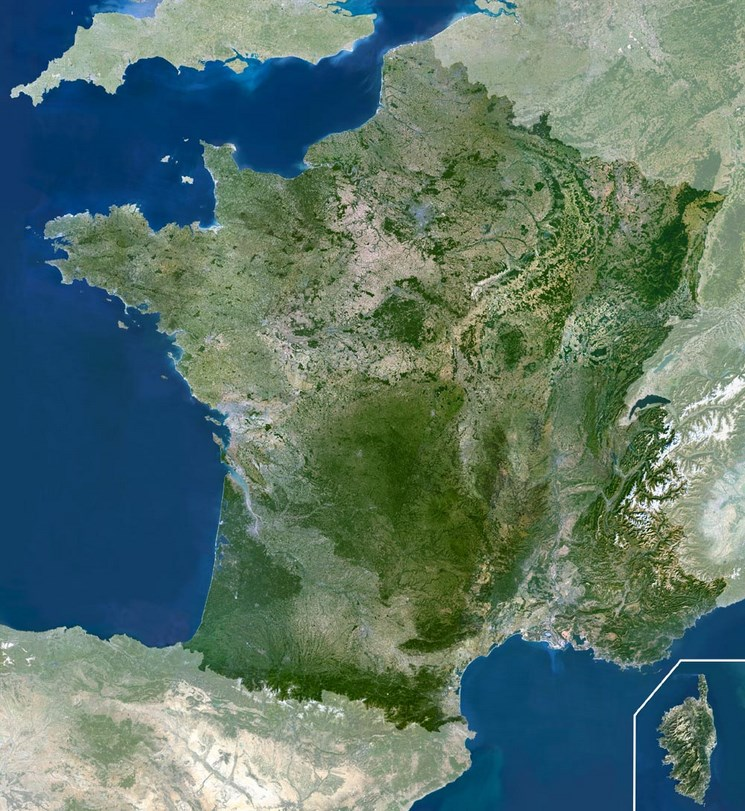
\includegraphics[scale=0.09]{figures/lib/france_satellite.jpg}};
    \path (modele) -- +(4.7,0) node[align=center] {Système modélisé};

   \draw[->] (carte) -- +(3.3,0) node[midway,above] {Représente} node[midway,below]{$\mu$};
   \draw[->] (carte) -- +(-3.2,0) node[midway,above] {ConformeÀ}  node[midway,below]{$\chi$};
\end{tikzpicture}
